\documentclass{article}

\usepackage[letterpaper, portrait, margin=1.5in]{geometry}

\usepackage{fancyhdr}
\usepackage{ragged2e}
\usepackage{graphicx}
\usepackage{caption}
\usepackage{amsmath}
\usepackage{rotating}
\usepackage{caption}
\usepackage{subcaption}

\usepackage{listings}
\usepackage{color}

\definecolor{dkgreen}{rgb}{0,0.6,0}
\definecolor{gray}{rgb}{0.5,0.5,0.5}
\definecolor{mauve}{rgb}{0.58,0,0.82}

\lstset{frame=tb,
  language=Java,
  aboveskip=3mm,
  belowskip=3mm,
  showstringspaces=false,
  columns=flexible,
  basicstyle={\small\ttfamily},
  numbers=none,
  numberstyle=\tiny\color{gray},
  keywordstyle=\color{blue},
  commentstyle=\color{dkgreen},
  stringstyle=\color{mauve},
  breaklines=true,
  breakatwhitespace=true,
  tabsize=4
}

\setcounter{secnumdepth}{1}

\usepackage{chngcntr}
\counterwithin{figure}{section}

\renewcommand*{\thepage}{C\arabic{page}}

\pagestyle{fancy}
\lhead{ACME Robotics}
\chead{\#8367}
\rhead{\ifcontents Contents \else Week \thesection \fi}

\newif\ifcontents
\contentstrue

\makeatletter
\renewcommand{\@seccntformat}[1]{}
\makeatother
\begin{document}

\subsection{X-Rail Mounting}
%! Mount the X-Rail.
This week the inner drive plates were cut. However, since the outer plates were not cut, the X-rail could not be mounted. As such, a stop-gap method was used to mount the X-Rail. While technically the X-rail was mounted before on Tetrix, it hardly worked. This meant that if the team wanted to have a functioning robot, they would need to create one that worked better. ACME wanted to meet a deadline for having the robot able functioning so it was important to make this stop-gap solution. Jon was assigned to create this. The easiest way to do this seemed to be by drilling mounting holes into two sheets of aluminum and folding them. It was important that the mounting solution be simple and quick to make because the deadline that the team needed to have a functioning robot by was fast approaching. 

\begin{figure}[h!]
\centering
\begin{subfigure}{.5\textwidth}
  \centering
  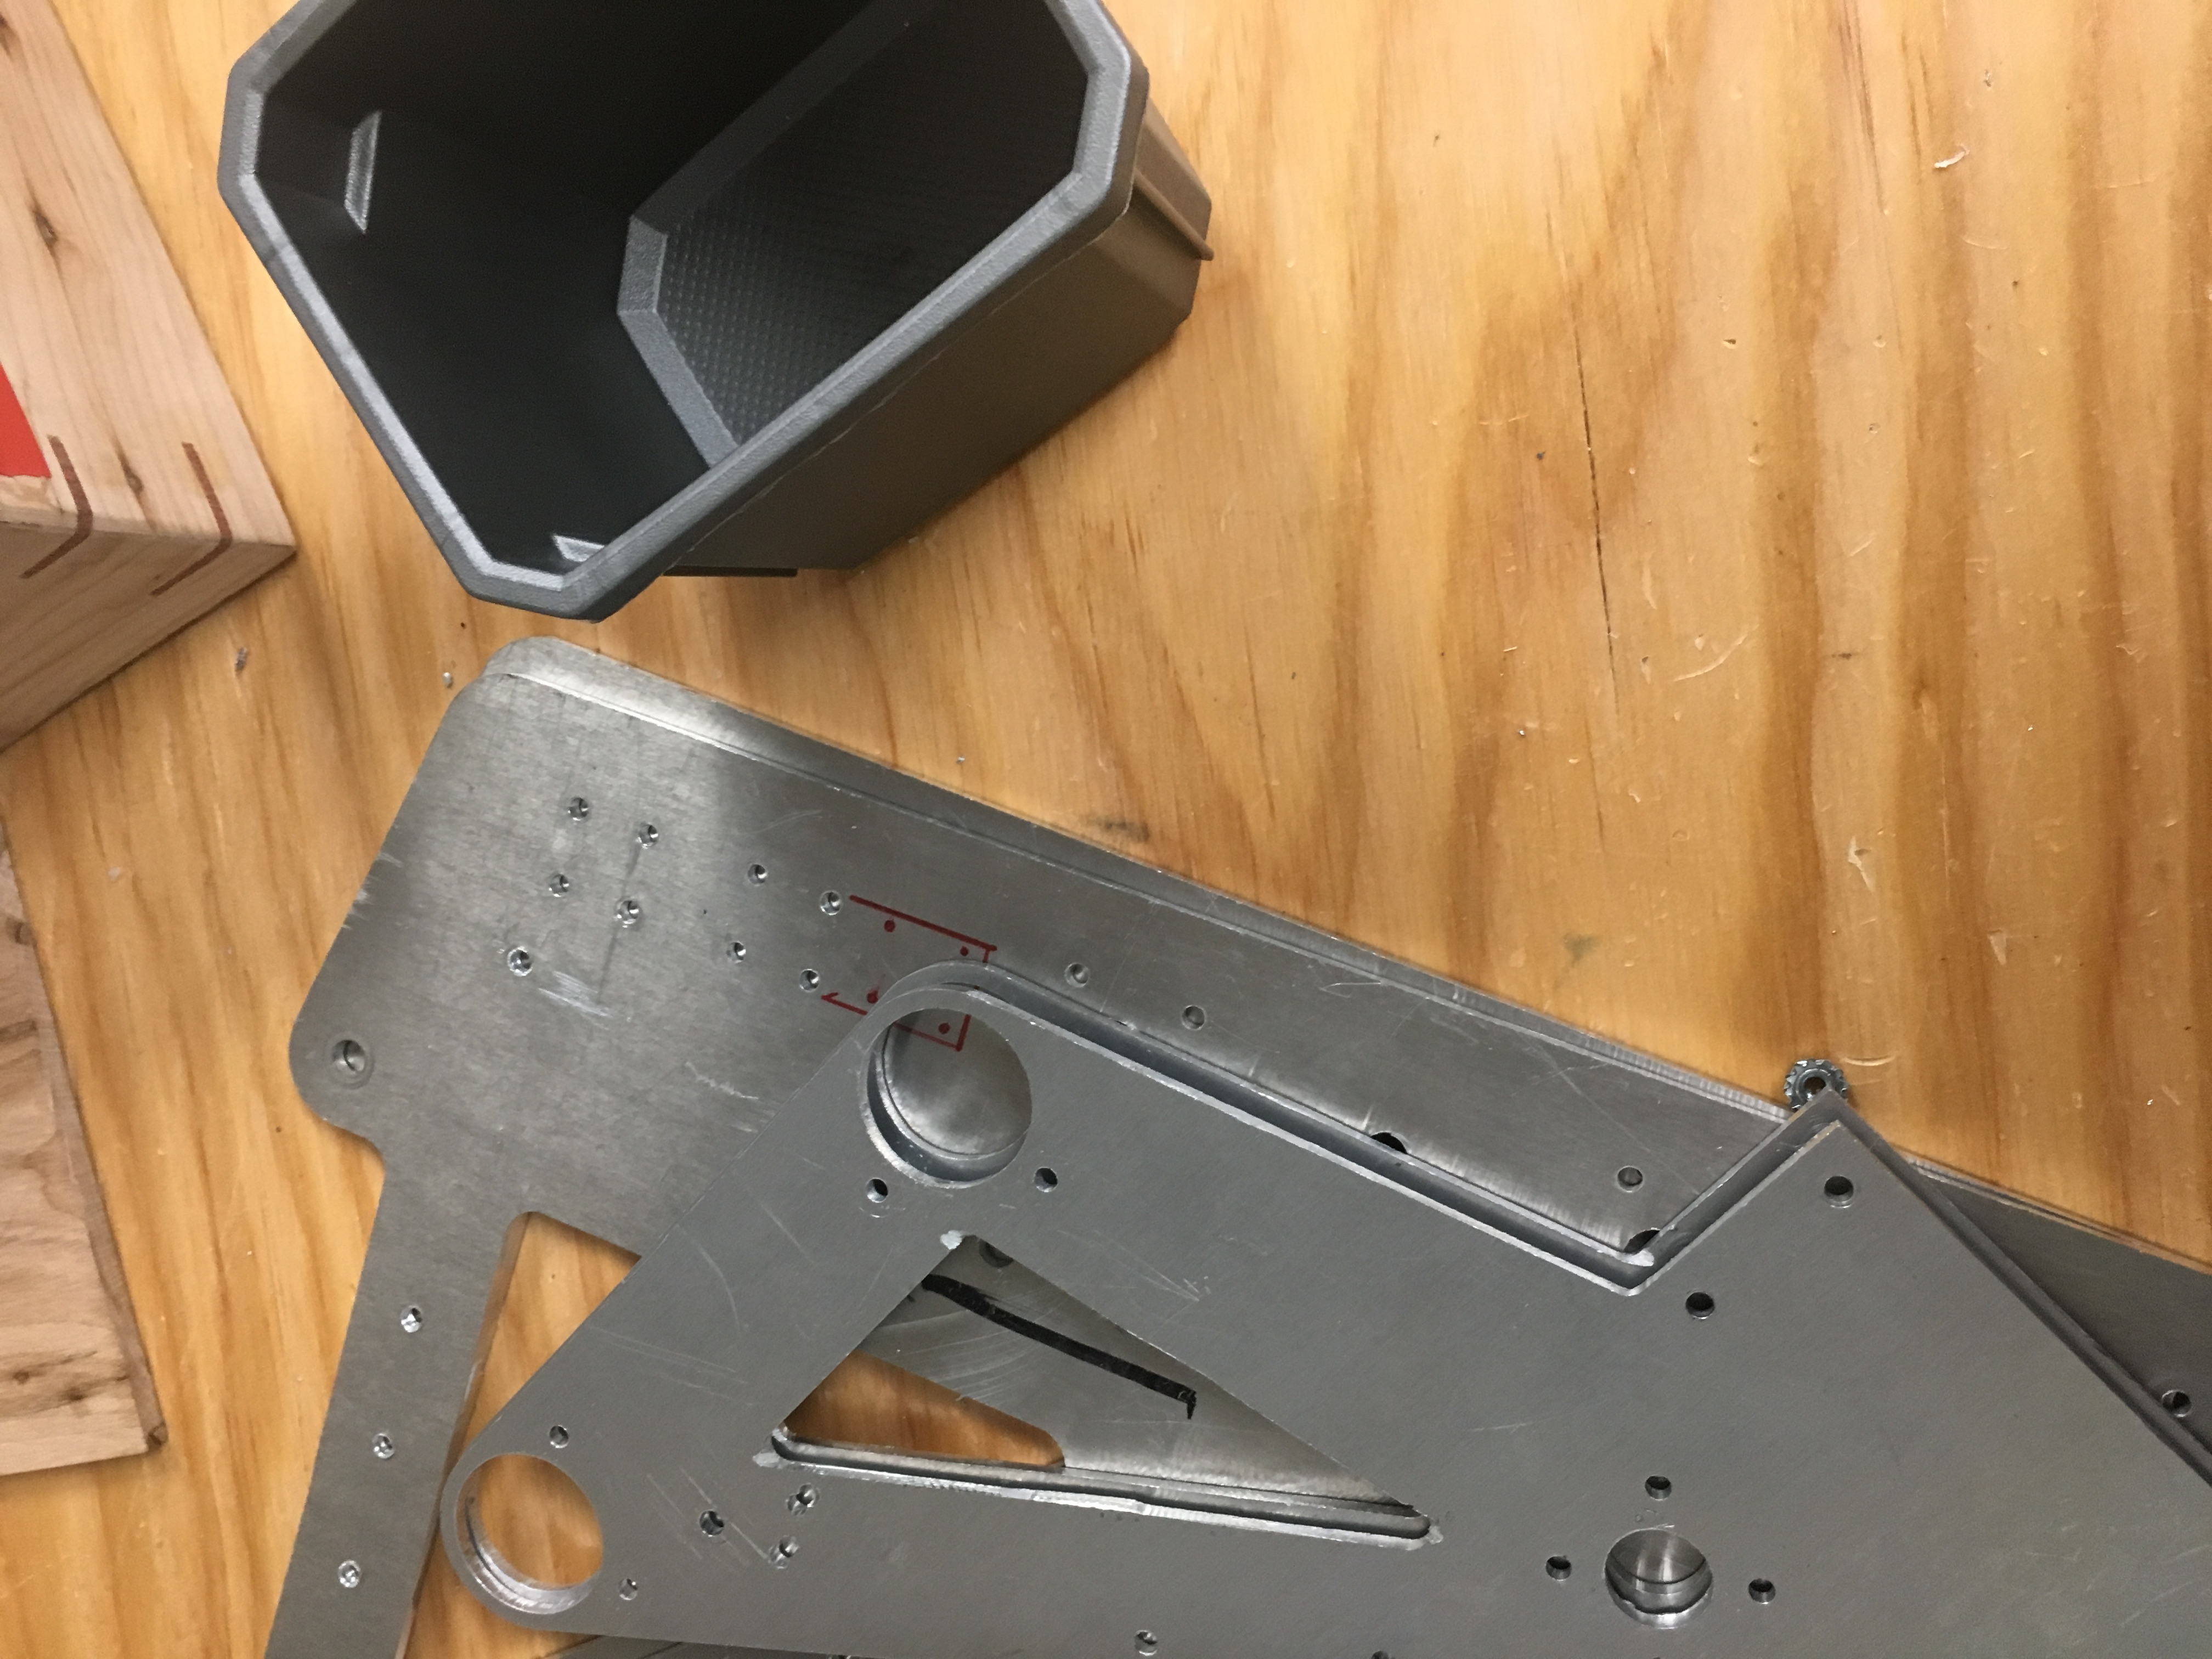
\includegraphics[width=\textwidth,angle=-90]{17_12-24/images/DrivePlates.JPG}
  \caption{Drive-Plates}
  \label{fig:Plates}
 \end{subfigure}
\begin{subfigure}{.45\textwidth}
  \centering
  \includegraphics[width=\textwidth]{17_12-24/images/Laguna.jpg}
  \caption{Cutting Drive-Plates}
  \label{fig:Cutting}
  \end{subfigure}
  \caption{Cutting New Drive-Train}
  \end{figure}

\subsection{Cutting Drive plates}
%!Setting up and cutting inside drive-plates
For the cutting processed we decided to use a CNC laguna, for its precision and accuracy rather than by hand or CNC plasma cutter.The job set up was pretty simple since we had been walked through it the previous time. The set up entailed us, to cut out two pockets two feet by 1 foot so as to allow our aluminum when screwed down, to rest flush with the top of the spoil board. We then orientated the board so that the bottom left corner of the board was at the X \& Y zeros, to allow for an easy tool path set up in Aspire. As an extra precaution in Aspire, tabs were added to the material that would be completely cut out, so that the router wouldn't throw the loose aluminum pieces. Since this plate was modeled to have precise mounting holes, it required us to make two tool changes, not hard to do in the program, but required us to learn a new step, Tool Touch offs. When we had finished the program portion of the set up we moved back to the Laguna, were we started with setting our X,Y \& Z zero's. The Z zero had to be set to the bottom of the pocket because the Laguna cuts from the bed surface not from the material. Those zeros are very important to get as accurately as possible, because the tool switches and touch offs are based on the first bit and the said zeros. After we made sure everything was set up to the best of our ability, we began cutting, about half through the first pass on the profile the 1/4 O-flute bit snapped due to depth and side impact on the bit. We quickly switched the bit and reset all our zeros and tool touch offs, then resumed the cut. We later talked to a professional, who told us that the bit we were using was for 1/16th inch aluminum not 1/8th, so we ended up buying a new one to replace theirs.  


\end{document}